\documentclass[11pt]{article}

\usepackage[a4paper,margin=1.5in]{geometry}
\usepackage[strict]{changepage}
% \usepackage[scale=0.92]{tgschola}
% \usepackage{fouriernc}
\usepackage{lmodern}
% \usepackage{libertinus}
\usepackage{inconsolata}
\usepackage[T1]{fontenc}

\usepackage{booktabs, threeparttable, adjustbox, tabularx, longtable}
\usepackage{amsmath, amssymb, amsthm, bbm}
\usepackage{hyperref, achicago}
\usepackage{caption, graphicx}
\usepackage{secdot, sectsty}
\usepackage{pdflscape}
\usepackage{placeins}
\usepackage{xcolor}
\usepackage{titling}

\usepackage[backend=bibtex, style=authortitle, citestyle=authoryear-icomp, maxcitenames=2, url=false]{biblatex}
\addbibresource{Lottery.bib}

\linespread{1}
\urlstyle{tt}

\sectionfont{\centering\normalfont\normalsize\scshape}
\subsectionfont{\centering\normalfont\normalsize\selectfont\itshape}
\subsubsectionfont{\centering\normalfont\normalsize\selectfont\itshape}

\sectiondot{subsection}

\renewcommand{\abstractname}{\vspace{-\baselineskip}}

\renewcommand\thesection{\Roman{section}}
\renewcommand\thesubsection{\thesection.\Alph{subsection}}
\renewcommand\thesubsubsection{\thesubsection.\arabic{subsubsection}}

\newcommand{\specialcell}[2][c]{\begin{tabular}[#1]{@{}c@{}}#2\end{tabular}}
\renewcommand{\today}{\ifcase \month \or January \or February \or March \or April \or May  \or June \or July \or August \or September \or October \or November \or December \fi \number \year}

\begin{document}

\title{\textsc{Using Lotteries to Encourage Saving: Experimental Evidence from Kenya}\protect\footnote{We are grateful to the study participants for generously giving their time. We thank Jonathan Page and Arun Varghese for invaluable research assistance. This study was pre-registered with the AEA RCT registry (AEARCTR-0000893). Files for replication are available at \url{https://github.com/princetonbpl/akiba-lottery-pub}.}}

\author{
	Justin Abraham
		\thanks{Department of Economics. University of California, San Diego. \protect\href{mailto:jabraham@ucsd.edu}{\nolinkurl{jabraham@ucsd.edu}}.},
	Merve Akbas
		\thanks{Department of Economics. Duke University. \protect\href{mailto:merve.akbas@duke.edu}{\nolinkurl{merve.akbas@duke.edu}}.},
	Dan Ariely
		\thanks{Fuqua School of Business. Duke University. \protect\href{mailto:dan@danariely.com}{\nolinkurl{dan@danariely.com}}.}, and
	Chaning Jang
		\thanks{The Busara Center for Behavioral Economics. \protect\href{mailto:chaning.jang@busaracenter.org}{\nolinkurl{chaning.jang@busaracenter.org}}.}
}

\maketitle

	\begin{abstract}

		We conduct a field experiment that randomly assigned 311 informal residents of Nairobi to either a prize-linked savings account (PLS)---a product that incorporate stochastic returns to deposits---against standard, interest-bearing accounts of equivalent expected value. In the PLS treatment, individuals could only enter the lottery conditional on their making a deposit. We implement a third treatment arm that provides feedback on lottery results unconditionally to test for regret aversion. Individuals saving with PLS with feedback made 42\% more deposits on average over the project period than participants who received a fixed incentive of equal expected value. We do not observe any effects of the lottery incentive on the amount deposited with PLS or on savings with other products. Lastly, we document limited evidence that use of PLS results in a 15\% increase in gambling activity. We argue that the effects on deposit frequency are due to regret aversion, a hypothesis which receives support from the presence of larger treatment effects conditional on winning the lottery but being unable to claim the prize.

		% be more explicit about third treatment
		% what's the motivation for testing the PLS?
		% edit this after reframing the paper

		\medskip \noindent
		JEL Classifications: D14, E21, G11

 	\end{abstract}

\newpage

\section{Introduction}

	% I will list three characteristics: (1) the importance of the question and of the main results; (2) the  clarity,  organization,  and  length  of  the  paper;  and  (3) its degree of novelty in either method or data.

	% The AEJ way is to talk policy, intervention, then mechanisms
	% need to delineate specific contributions to each literature
	% on PLS: mechanisms
	% on regret aversion: dynamics

	% consider switching so that first preview results and then talk about literature/contributions: summary of experiment and PLS result, introduce regret confound, summary of regret result, long term regret result, result on other savings and gambling, contribution to PLS, contribution to regret aversion

	% consider talking in length about mechanisms in the results section 

	% Somville structure: introduce default effect, statement of empirical contribution, empirical strategy, hypothesis then preview of results, interpretation of results, contributions/literature

	% Schaner structure: policy motivation, experiment, results preview, mechanism/interpretation, contributions/literature

	The ability to save is one of the most important avenues toward economic development; it provides a means to smooth consumption under incomplete insurance and it makes possible productive investments in the presence of credit constraints. There exists, however, a host of obstacles that prevent poor households from accruing savings to their advantage. There are supply-side limitations to formal finance, such as high initial and transaction costs, that may be prohibitive for the poor. As a result, they often have to resort to methods of saving that can be costly and have limited functionality \parencite{collins_portfolios_2009,karlan_savings_2014,banerjee_economic_2007,schaner_cost_2011}. 

	On the demand side, knowledge gaps, mistrust of financial institutions, and behavioral biases prevent the poor from saving as much as they would like. In Kenya, around 80\% of adults have an account with a financial institution or mobile money yet only 30\% report using them to save \parencite{demirguc-kunt_global_2018}. Policies that target costs on the supply side are known to increase account ownership but have been less effective at encouraging usage \parencite{dupas_why_2013,karlan_banking_2016}. Meanwhile, savings products designed to address behavioral barriers have been shown to be extremely cost-effective, especially compared to direct subsidies.\footnote{\textcite{karlan_price_2018} estimate very low interest rate elasticities and limited impacts of easing account ownership requirements. \textcite{schaner_persistent_2018} boost short-run individual savings by USD 1.38 with rates of up to 20\%.} Track-keeping objects \parencite{akbas_how_2016}, SMS reminders \parencite{karlan_getting_2010}, and default contributions \parencite{thaler_save_2004,chetty_active_2014,somville_saving_2018} which address undersaving due to limited attention. Binding commitment devices, in the form of account restrictions \parencite{ashraf_tying_2006} or the application of social pressure \parencite{dupas_why_2013}, can help individuals with time-inconsistent behavior follow through on saving. This literature has demonstrated the importance of product design or \textit{choice architecture} in financial decisionmaking.

	This article examines the potential of prize-linked savings (PLS)--- a savings product that incorporate lottery-like payoffs---in encouraging saving. The key novelty of PLS accounts is that users receive a stochastic payoff in addition to, or in lieu of, certain interest payments. Common among PLS products is that consumers face no risk of negative returns, at least guaranteeing the full principal amount. PLS have been in use since at least the 18\textsuperscript{th} century and presently exist in various forms around the globe \parencite{murphy_lotteries_2005,kearney_making_2010}. Any kind of savings product that allows consumers to enter raffles or earn lottery tickets conditional on deposits may be considered PLS. NS\&I Premium Bonds in the U.K., the now-defunct ``A-Million-A-Month'' Account in South Africa are prominent examples of this type of savings product.

	We conducted a laboratory and field experiment to analyze the effects of PLS on savings behavior over time. We provided a mobile savings product to 311 informal residents in Nairobi, Kenya and observed account activity over a 60-day period. Using mobile savings allowed us to minimize transactions costs and to collect detailed data on individual transactions. Roughly one-third of our sample was randomly assigned a savings account which matched contributions at 5\%. A second group was assigned an account that yielded stochastic returns equal in expectation to the 5\% match through a daily lottery. Each day, participants received a lottery ticket whose earnings were proportional to amount saved that day instead of a certain match. We compared the match and lottery groups to determine how PLS impacts savings behavior. We find that participants using PLS made 42\% more deposits on average over the project period than participants receiving the matching incentive. This amounts to 5-6 additional days that treated participants made deposits to their savings account. We find no effect of PLS on total amount saved, a finding largely consistent with earlier experimental results. Consequently, we find no evidence that PLS displaced savings from other sources. On gambling behavior, we find that participants who used PLS with feedback reported higher gambling activity 15 percentage points more than the control group.

	There are a host of theoretical explanations behind the apparent demand for PLS as opposed to standard savings. Our second objective is to quantify the role of regret aversion \parencite{bell_risk_1983,loomes_regret_1982} as a specific mechanism driving our treatment effects. Regret theory refers to a class of behavioral models that posit that individuals minimize anticipated regret arising from the comparison of prospects against foregone outcomes. In the context of uncertainty, regret aversion has been shown to promote apparently risk averse and risk-seeking behavior  \parencite{zeelenberg_consequences_1996}. 

	To test for regret aversion, we implemented a third treatment wherein participants received the same PLS account with the additional feature that they received a lottery ticket and observed the lottery results only after they had made a deposit that day. That feedback about hypothetical lottery results affects decisions to save is a central prediction of regret aversion. We find that when the resolution of lotteries depends on saving, the effect of PLS on deposits is 20\% smaller than when feedback is always given. In other words, participants assigned to PLS with feedback are motivated to save (and enter the lottery) in anticipation of regret they may feel from having a winning ticket but not being able to claim the prize. Exploiting the longitudinal nature of our data, we also find that recent experiences of regret increase the likelihood of making a deposit in subequent days by 8\%. Together, our evidence points to the importance of regret aversion in demand for PLS.

	This study is one of the first field experiments conducted on PLS in a low-income setting. Two laboratory studies provide evidence of a positive effect of stochastic returns on saving. \textcite{atalay_savings_2014} conducted an online portfolio-choice experiment that resulted in participants saving an additional 12 percentage points more with lottery-linked and regular savings than with regular savings alone. Notably, participants who saw an increase in total savings shifted away from lottery expenditures and consumption rather than from regular savings. \textcite{filiz-ozbay_lottery_2015} found participants are more likely to delay payments with lottery-like returns compared to guaranteed interest of equivalent expected value. Outside the laboratory, evidence surrounding PLS is more limited. Our study comes closest to \textcite{gertler_long-term_2017}, which studies the long-term effects of PLS in Mexico. They found that bank branches offering PLS saw 41\% more account openings and that these continued to be used five years after the lottery incentives expire. \textcite{loibl_testing_2016} conducted a randomized evaluation of IDAs in the U.S. that incorporated a lottery-based savings match. That study found no significant effect of the program relative to guaranteed matching, even when it was bundled with reminder calls and frequent deposit deadlines. They attribute the result to liquidity constraints among their sample, which potentially precluded the benefits of behavioral interventions. Lottery-based incentives applied in other domains, including labor supply \parencite{brune_effect_2015} and health-related behaviors \parencite{kimmel_randomized_2012,bjorkman_nyqvist_using_2015}, are found to have significant effects. We contribute to this line of research by testing for and quantifying the role of regret aversion as an underlying behavioral mechanism.

	Our experiment also joins a strand of the behavioral literature studying the applicability of regret aversion. \parencite{zeelenberg_consequences_2004} is a cross-sectional study of Dutch lotteries that showed that feedback about winnings in one lottery elicits feelings of regret and that it influences decisions to play.  \parencite{filiz-ozbay_auctions_2007} finds evidence that regret felt by bidders who lose can explain overbidding in first price auctions. As in this study, they utilize the manipulation of feedback about the winning bid to test for regret aversion. The present study contributes to this literature in examining the implications of regret aversion in repeated settings. Namely, we find evidence that regret aversion appears more intense among those who recently experienced regret. A recent paper by \textcite{imas_regret_2016} argues that regret aversion results in an \emph{undervaluation} of lotteries in repeated settings because frequent experiences of regret may dissuade individuals from making risky choices and because feeadback provides individuals the opportunity to learn about the incentives. Regret aversion in repeated settings remain a largely unexplored area of research.

	The remainder of the paper is structured as follows. Section \ref{sec:design} describes our experimental design, Section \ref{sec:est} outlines our estimation strategy, Section \ref{sec:results} discusses our main results, and Section \ref{sec:conclusion} concludes.

% \section{Related Literature} \label{sec:litreview}

	% this section should discuss previous literature: competing explanations for gambling and what they predict
	% demand for PLS and recent experimental evidence
	% theories of regret
	% generally, unanswered questions

		% why people insure and gamble is a longstanding economic puzzle wiwth many explanations coming to fore to explain it
			% friedman savage, machina's paradox
		% can classify theories into three main categories
			% preferences for skewness
			% subjective probabilities
			% specific to developing settings: as a form of saving
		% what are the implications of believing one over the other?
			% what are the behavioral predictions and how do empirical regularities match up?
		% theoretically, this is why PLS are promising

		% why is theory of regret important in the first place? (why did we choose to test it?)
		% what are the prevailing theories of regret?
		% how does this relate to gambling?
		% what are the behavioral predictions and how do empirical regularities match up?

		% experimental paragraph as-is with lybbert and gertler
		% explain unanswered questions and tie it back to the present study

	% How might lotteries induce savings? Preferences for skewed returns are well-documented, so the use of lottery-like structures may play a viable role in incentivizing savings. Models departing from expected utility theory incorporate the overweighting of small probabilities \parencite{kahneman_advances_1992} and attention to salient payoffs \parencite{bordalo_salience_2012} in order to account for seemingly risk-loving behavior among risk-averse individuals. Research on preferences for skewness have produced a litany of potential explanations for this phenomenon.\footnote{This paper does not test against these competing explanations and introduces them as a framework for interpreting results.} One broad strand of the literature understands the overweighting of long-odds as a result of persistent preferences for such gambles. Playing the lottery may provide excitement from taking risks and a chance to win a large payoff \parencite{conlisk_utility_1993}. Similarly, aversion to anticipated regret from foregoing a big prize could drive gambling behavior \parencite{loomes_regret_1982,zeelenberg_consequences_2004}. Credit-constrained households may also rely on lotteries to save for large, indivisible expenditures \parencite{kwang_why_1965,herskowitz_gambling_2016}. Alternatively, preferences for gambling may result from bias in subjective probabilities vis-\`{a}-vis true probabilities. The biased weighting of probabilities implies more fickle gambling behavior that depend on exposure to information and repeated choice \parencite{hertwig_descriptionexperience_2009}.

	% two types: biases in subjective probabilities or preference for skewness
		% bias hypothesis predicts that people can learn over time "debiasing"
		% preference hypothesis predicts no learning
	% explain and elaborate hot-hand and gambler's fallacy
	% Extensive research has tried to explain the higher demand for lotteries and gambling among people with lower income. One approach allows individuals to use subjective probability weighting to over-weight low probability events, e.g. rank-dependent expected utility theory (Quiggin, 1982); cumulative prospect theory (Tversky and Kahneman, 1992). Another approach, skewness, allows utility to depend upon both absolute and relative wealth so that lotteries offer an opportunity to move up in terms of relative wealth (Shefrin and Statman, 2000). Crossley et al. (2011) suggest that people can use lotteries to convexify their budget sets.
	% what is the link to regret aversion? the first point has to do with risk attitudes the second point has to do with violations of independence
	%  The Probability Weighting Function (Drazen Prelec )
	% check lit review in the notes section
	% bilal zia paper on debiasing
	% The Utility Analysis of Choices Involving Risk  friedman savage

	% check out brune literature review for empirical evidence in labor, medicine, etc.
	% check out new work by gertler and zia on this
	% Discuss \parencite{dizon_leveraging_2016}
	% is it reasonable to assume banks are risk neutral?
	% should check whether different results are being driven by regret aversion (would people have been aware that others were winning?)
	% where should we state our priors?
	% regret aversion + CPT = regret affects the reference point https://voxeu.org/article/regret-and-economic-decision-making

\section{Experimental Design} \label{sec:design}

	\subsection{Sampling Frame}

		We conducted our experiment in conjunction with the Busara Center for Behavioral Economics with 311 participants recruited from Nairobi's low-income neighborhoods. Three quarters of our sample reside in Kibera, the city's largest informal settlement. We drew a random sample of participants over 18 years old using SMS and phone calls from the Busara Center's active pool of over 11,000 Nairobi residents. Nearly 60\% of our sample is female with a median age of 28 years. Less than half of the participants in our sample reported that they are employed with only 5\% reported receiving a regular income. The employed in our sample largely work in retail or are students. The median PPP-adjusted monthly income among those employed is USD 77.\footnote{Monetary payouts were in Kenyan shillings (KES). We report USD values calculated at purchasing power parity using a conversion factor for private consumption of 38.15 in 2013. The price level ratio of PPP conversion factor (GDP) to KES market exchange rate for 2011 was 0.444.}

		Approximately 55\% of our sample saves regularly with a majority of savers utilizing rotating savings and credit associations (ROSCA), a type of informal group savings. The average stock of savings among these individuals amount to USD 23. A significant fraction of savers also report using M-Shwari, a mobile service that provides a lockbox account and offers short-term credit.\footnote{The savings product we designed is comparable to M-Shwari in that it also offered commitment savings and a 5\% return on deposits.} Mobile transactions are made with M-Pesa, an SMS-based money system made accessible by the ubiquity of mobile phones in Kenya.

		The surge of mobile phone usage in Kenya has allowed the recent popularity of mobile sports betting. SportPesa, one of the most popular mobile gambling services, reports over 800,000 registered users as of 2015 \parencite{kemibaro_sportpesa_2015}. In our sample, 24\% of participants at baseline report that they have some problem with gambling. 11\% of participants report that they gamble at a casino, bet money at racetracks or sporting events, played the sweepstakes, or played cards for money daily or more frequently in the last 12 months.

		% what do peopl save for? how long does this take? could affect what we see in this setting
		% there are better references on mobile gambling in kenya \textcite{herskowitz__2016}

	\subsection{Data Collection}

		Participants were first invited to the lab at the Busara Center where they completed a computerized questionnaire and behavioral tasks. Experimental sessions included up to 25 participants at a time and were administered in English by research assistants. The following outlines the schedule of tasks during the lab portion of the study:

		\begin{enumerate} \setlength{\itemsep}{1pt}
		\item Coin toss task \parencite{eckel_sex_2002}\footnote{This elicitation method produces interval estimates of the coefficient of relative risk aversion, $\rho$, under the assumption of constant relative risk aversion. We take the midpoint of the upper and lower intervals as point estimates. For participants with $\rho \geq 3.46$ and $\rho \leq 0$, we use boundary values as point estimates.}
		\item Titration task for temporal discounting \parencite{cornsweet_staircase-method_1962}
		\item Willingness-to-pay to play a lottery
		\item Candian Problem Gambling Index \parencite{ferris_canadian_2001}
		\item Internal locus of control \parencite{rotter_generalized_1966}
		\item Demographics questionnaire
		\end{enumerate}

		At the conclusion of the demographics questionnaire, participants received KES 200 for completing the session and an additional KES 50 for arriving on time. Lab sessions took place over five weeks in May and June of 2014. We refer to this period before beginning the savings program as the baseline.

		Following the lab session, participants were enrolled in the 60-day savings program and randomly assigned to one of three incentive schemes: one fixed match and two lottery-based matches. Savings incentives are detailed in Section \ref{sec:treat}. Each participant received KES 20 airtime credit and asked to practice saving using Sambaza. Participants then received business-card sized handouts which described their savings program and bonuses. We provided participants simple instructions for saving and listed the number to our project phone. This was the number through which the savings program operated that also functioned as a help line for participants.

		All participants completed the savings program by August 2014. In September 2014, we called participants and conducted an endline survey that included questions on outside savings, gambling activity, and program feedback. We obtained endline surveys for all but 27 of the 311 participants. We find no evidence that completion of the endline survey correlates with treatment assignment.

		\clearpage

	\subsection{Mobile Savings Product}

		We implemented our 60-day mobile-phone savings program over Safaricom's Sambaza airtime sharing service. Using Sambaza, Safaricom users can send airtime to each other free of charge. Participants saved into our program by sending airtime to a designated project phone that held the airtime in an account for each user.

		Participants received two SMS messages every morning after the first morning of the project period. The first message arrived at 8:00 daily summarizing how much the participant saved the previous day, how much the participant earned through a matching contribution or winnings, and their total balance. An hour later, participants received a beginning-of-day message encouraging them to save that day. Participants were allowed to send in savings at any time but any savings sent in after first message with the lottery results would be counted towards the next day's total. We used a custom-developed administrative system to manage the savings program. This system logged airtime sent to our project phone, maintained an internal ledger of balances, sent automated SMS confirmations after every transaction, and conducted the daily lottery game.

		Participants enrolled in the savings program for two consecutive periods of 30 days starting from the day of a participant's lab session. On a participant's 30th day, a field officer called them and asked if they wished to withdraw any amount of their balance. Participants who requested withdrawals were sent tranfers equal to their plus a withdrawal fee compensation. The product we provided was a ``lockbox'' account where regular withdrawals outside of this opportunity were prohibited.\footnote{This feature is commonplace among informal savings and is increasingly incorporated into savings interventions. \textcite{ashraf_tying_2006} provides evidence that commitment savings increases long-term savings among women who exhibit present-biased time preferences. Commitment savings may also be advantageous when intrahousehold bargaining hinders saving \parencite{banerjee_economic_2007,schaner_cost_2011}.} Transfers were made using the mobile money system M-Pesa to minimize transaction costs. M-Pesa accounts are associated with a SIM card and transactions are made via SMS. Participants could deposit and withdraw money from the account at any of more than 10,000 agents throughout Kenya, including those located in the informal settlements where our participants reside.

		Participants were called and notified a few days before the end of their second 30-day period that the program would be ending soon. After receiving the end-of-day message on their 60th day, participant were unenrolled from the program and were no longer allowed to save. Field officers called participants to confirm final balances and sent M-Pesa transfers equal to total balances net of withdrawals shortly after. Participants paid no explicit fees to participate in our program.

	\subsection{Treatment} \label{sec:treat}

		Participants enrolled in the savings program were randomized into one of three different incentive schemes. Tables \ref{tab:sum-ysumall} reports summary statistics and tests for balance across treatment groups of several pre-treatment characteristics. We find no overall imbalance based on a test of joint significance across all observables.\footnote{We account for the correlation of treatment to usage of a savings account in Section \ref{sec:est}.}

		\begin{enumerate} \setlength{\itemsep}{1pt}

			\item \textit{Matching contributions:} Participants in the matching group earned a 5\% matching contribution on any amount that they saved on a particular day. The match was automatically added to the mobile account. The amount of the incentive and the participants' daily balance were reported every morning via SMS. We take this group as our control group.

			\item \textit{Prize-linked savings with feedback:} Every day, participants earned a lottery ticket transmitted via SMS that could win a cash prize in proportion to the amount they saved on the same day.

			A lottery ticket was a random sequence of four numbers between 1 and 9, inclusive. Each morning, our administrative system randomly generated a winning sequence of four numbers. Prizes were awarded according to how well a participant's lottery numbers matched the winning numbers. If the first or second numbers matched, a 10\% match of savings was awarded. If both the first and second numbers matched, a 100\% match of savings was awarded. Finally if all numbers matched, a prize of 200 times the daily savings was awarded. The expected earnings on this lottery ticket were equal to the 5\% match earned in the control group---\textit{i.e.} the expected payoffs were equivalent but by a mean-preserving increase in risk.

			Our system entered winnings into the internal ledger and reported lottery results via SMS the following day. Participants with winning lottery tickets who did not save could not claim the prize but received feedback on their lottery results daily. We henceforth refer to this group as the PLS group. 

			\item \textit{Prize-linked savings without feedback:} This scheme is identical to the Lottery treatment except participants in this third group only received lottery tickets and made aware of their potential winnings if they made a non-zero deposit the previous day. We henceforth refer to this group as the No Feedback group.

		\end{enumerate}

		\begin{table}[h]\centering \def\sym#1{\ifmmode^{#1}\else\(^{#1}\)\fi} \caption{Baseline balance by treatment group} \label{tab:sum-ysumall} \maxsizebox*{\textwidth}{\textheight}{ \begin{threeparttable} \begin{tabular}{l*{5}{c}} \toprule
          &\multicolumn{1}{c}{(1)}&\multicolumn{1}{c}{(2)}&\multicolumn{1}{c}{(3)}&\multicolumn{1}{c}{(4)}&\multicolumn{1}{c}{(5)}\\
          &\multicolumn{1}{c}{\specialcell{No Feedback -\\Control}}&\multicolumn{1}{c}{\specialcell{PLS -\\Control}}&\multicolumn{1}{c}{\specialcell{No Feedback -\\PLS}}&\multicolumn{1}{c}{\specialcell{Control mean\\(SD)}}&\multicolumn{1}{c}{Obs.}\\
\midrule
Female    &     0.07&     0.10&     0.03&     0.52&      311\\
          &   (0.07)&   (0.07)&   (0.07)&   (0.50)&         \\
Age       &     0.78&     0.72&    -0.05&    30.75&      311\\
          &   (1.39)&   (1.34)&   (1.35)&   (9.83)&         \\
Completed std. 8&    -0.02&    -0.02&     0.00&     0.99&      311\\
          &   (0.02)&   (0.02)&   (0.02)&   (0.10)&         \\
Married/co-habitating&     0.10&     0.09&    -0.01&     0.42&      311\\
          &   (0.07)&   (0.07)&   (0.07)&   (0.50)&         \\
No. of children&     0.23&     0.24&     0.01&     1.75&      311\\
          &   (0.24)&   (0.25)&   (0.25)&   (1.70)&         \\
Currently saves&     0.05&    -0.10&    -0.15&     0.56&      311\\
          &   (0.07)&   (0.07)&   (0.07)&   (0.50)&         \\
Total savings last month&   -17.81&    -7.04&    10.77&    58.82&      311\\
          &  (11.88)&  (12.55)&   (9.23)& (106.26)&         \\
Monthly income&    -3.68&    -0.59&     3.09&   112.05&      311\\
          &  (17.63)&  (16.85)&  (15.46)& (137.13)&         \\
Employment status&     0.05&    -0.03&    -0.08&     0.50&      311\\
          &   (0.07)&   (0.07)&   (0.07)&   (0.50)&         \\
Coefficient of relative risk aversion&     0.08&    -0.03&    -0.12&     1.16&      311\\
          &   (0.18)&   (0.17)&   (0.18)&   (1.27)&         \\
Locus of control&     0.48&    -0.83&    -1.31&    69.81&      311\\
          &   (1.40)&   (1.46)&   (1.37)&  (10.78)&         \\
Standardized CPGI&    -0.11&    -0.22&    -0.11&    -0.00&      311\\
          &   (0.13)&   (0.12)&   (0.12)&   (1.00)&         \\
Exp. discount factor&    -0.05&    -0.01&     0.04&     0.33&      311\\
          &   (0.03)&   (0.03)&   (0.03)&   (0.20)&         \\
\midrule Joint test \emph{p}-value&     0.44&     0.72&     0.42&         &         \\
\bottomrule \end{tabular} \begin{tablenotes}[flushleft] \footnotesize \item \emph{Notes:} The first three columns report the difference of means across treatment groups with standard errors in parentheses. Column 4 reports the mean of the control group with SD in parentheses. The bottom row reports the \(p\)-value of a joint test of significance for each hypothesis. \end{tablenotes} \end{threeparttable} } \end{table}

% File produced by sum-treat.do with /Users/justin/Repos/akiba-lottery-pub/data/clean/akiba_wide.dta on 15:49:29 12 Aug 2020 by user justin on Stata 13.1 with seed X53d8cd0fc43f462544a474abacbdd93d00044a8f

		% consider writing a table with all of the features across treatment groups (lockbox, interest rate, reminder, lottery, feedback)

		\clearpage

\section{Empirical Strategy} \label{sec:est}

	% \subsection{Average Treatment Effect}

		We use the following reduced-form specification to estimate the treatment effect of lottery incentives on participant outcomes.

		\begin{equation} \label{eq:teffect}
			Y_{i} = \beta_{0} + \beta_{1}\text{NF}_{i} + \beta_{2}\text{PLS}_{i} + \varepsilon_{i}
		\end{equation}

		$Y_{i}$ refers to the outcome variables for individual $i$ measured after the end of the savings program. NF$_i$ indicates assignment to the No Feedback group and PLS$_i$ indicates assignment to the PLS group. The omitted group is the control group. We test $\beta_{1} = 0$ and $\beta_{2} = 0$ to identify the effects of PLS and PLS without feedback relative to the control group. We additionally test $\beta_{2} - \beta_{1} = 0$ for differential effects between the two PLS treatments. Standard errors are clustered at the individual level.

		To improve precision and to control for potential selection bias, we apply covariate adjustment with a vector of baseline indicators.\footnote{We include as control variables 1. Participant is female, 2. Participant is younger than 30 years old, 3. Participant completed primary school, 4. Participant is married, 5. Participant has at least one child dependant, 6. Participant uses a savings account, and 7. Above median CPGI score.} We obtain the covariate-adjusted treatment effect estimate by estimating Equation \ref{eq:teffect} including the demeaned covariate vector $\mathbf{X}_{i}$ as an additive term and as an interaction with the treatment indicator.

		\begin{equation} \begin{split} \label{eq:controls}
			Y_{i} = & \beta_{0} + \beta_{1}\text{NF}_{i} + \beta_{2}\text{PLS}_{i} + \mathbf{X}'_i \gamma_{0} \\
					& + \text{NF}_{i} \mathbf{X}'_i \gamma_{1} + \text{PLS}_{i} \mathbf{X}'_i \gamma_{2} + \varepsilon_{i}
		\end{split} \end{equation}

		The set of indicators partitions our sample so that our estimate remains unbiased for the average treatment effect \parencite{lin_agnostic_2013}. As in Equation \ref{eq:teffect}, we test $\beta_{1} = 0$ and $\beta_{2} = 0$ to identify the effects of the PLS with and without feedback relative to the matching group and test $\beta_{2} - \beta_{1} = 0$ for differential effects between the two PLS treatments. Standard errors are clustered at the individual level. Equation \ref{eq:teffect} is our preferred specification and report results with covariate adjustment for robustness.

		% either drop this section or discuss robustness in the results section

		We might expect that the errors of each outcome variable are correlated. Instead of estimating these equations separately, we estimate the system of seemingly unrelated regressions (SUR) to improve the precision of the coefficient estimates \parencite{zellner_efficient_1962}. SUR estimation is equivalent to OLS when the error terms are in fact uncorrelated between regressions or when each equation contains the same set of regressors. We perform joint estimation over outcome groups for Equation \ref{eq:teffect} and Equation \ref{eq:controls} separately.

		We control for the family-wise error rate (FWER) to correct for multiple inference. We compute adjusted $p$-values within categories of outcome variables using the free step-down resampling method \parencite{westfall_resampling-based_1993,anderson_multiple_2008}. This approach sets the size of the test to exactly the desired crticial value. We apply this correction over outcome variables in each family and separately for each hypothesis test. For each variable, we apply the procedure with 10,000 iterations and report both unadjusted and adjusted $p$-values.

	% \subsection{Minimum Detectable Effect Sizes}

	% 	To determine whether our null findings identify the absence of a true effect or signify a lack of statistical power, we report the minimum detectable effect size (MDE) for each outcome.

	% 	\begin{equation}
	% 		\mathrm{MDE}_{\hat \beta} = (t_{1-\kappa} + t_{\alpha/2}) \times \mathrm{SE}(\hat \beta)
	% 	\label{eq:mde} \end{equation}

	% 	This metric is the smallest effect that would have been detectable given our current sample size. Thus, a MDE greater than our estimated treatment effect suggests that null results are due to a lack of statistical power. We calculate MDEs \textit{ex post} with $\alpha = 0.05$ and 0.80 power for both No Feedback and PLS treatment effects.

	% 	% probably drop this section

	% \subsection{Heterogeneous Treatment Effects}

	% 	We analyze the extent to which the savings program produced heterogeneous treatment effects with the following specification.\footnote{$\beta$ here denotes a different parameter than those in the previous regressions.}

	% 	\begin{equation} \begin{split}
	% 	Y_{i} = & \beta_{0} + \beta_{1}\text{NF}_{i} + \beta_{2}\text{PLS}_{i} + \delta_{0}x_{i} \\
	% 				& + \delta_{1}(\text{NF}_{i} \times x_{i}) + \delta_{2}(\text{PLS}_{i} \times x_{i}) + \varepsilon_{i}
	% 	\end{split} \label{eq:heteffect} \end{equation}

	% 	$x_{i}$ is the binary dimension of heterogeneity measured before treatment assignment. $\delta_{1}$ and $\delta_{2}$ respectively identify the heterogeneous treatment effects of the two PLS products relative to individuals whose $x_{i} = 0$. Standard errors are clustered at the individual level. We estimate this model with the following baseline variables as $x_{i}$: gender, marriage status, below age 30, completed std. 8, uses a savings account, above median monthly income, employment status, above median CPGI score, coefficient of relative risk aversion, above median indifference point.

	% \subsection{Time-Varying Treatment Effects}
	%
	% 	Using detailed daily transaction data, we can estimate treatment effects of PLS conditional on the time elapsed since the start of the savings program. We estimate a model that interacts the treatment indicators with a linear time trend.
	%
	% 	\begin{equation} \begin{split}
	% 	Y_{i,t} = & \beta_{0} + \beta_{1}\text{NF}_{i} + \beta_{2}\text{PLS}_{i} + \lambda_{0}t \\
	% 				& + \lambda_{1}(\text{NF}_{i} \times t) + \lambda_{2}(\text{PLS}_{i} \times t) + \varepsilon_{i}
	% 	\end{split} \label{eq:timelinear} \end{equation}
	%
	% 	In this equation, $t$ is the number of days since the start of the savings program and $Y_{i,t}$ denotes whether participant $i$ made a deposit at period $t$. We also estimate this equation for $Y_{i,t}$ as the amount deposited in period $t$. $\lambda_1$ is the marginal effect of the lottery incentive on $Y_{i,t}$ with respect to days elapsed. $\lambda_2$ is the marginal effect of lottery with feedback. We test the hypotheses $\lambda_1 = 0$ and $\lambda_2 = 0$---that the effects of PLS are constant as a function of time. Standard errors are clustered at the individual level.
	%
	% 	Using detailed daily transaction data, we can estimate treatment effects of PLS conditional on the time elapsed since the start of the savings program. We estimate day-specific effects with the following specification.
	%
	% 	\begin{equation} \begin{split}
	% 	Y_{i,t} = & \beta_{0} + \beta_{1}\text{NF}_{i} + \beta_{2}\text{PLS}_{i} \\
	% 				& + \sum_{t=2}^{60} \bigg [ \zeta_{t} \tau_{t} + \eta_{t}(\text{NF}_{i} \times \tau_{t}) + \theta_{t}(\text{PLS}_{i} \times \tau_{t}) \bigg ] + u_{i, t}
	% 	\end{split} \label{eq:timedummy} \end{equation}
	%
	% 	$Y_{i, t}$ is the outcome for individual $i$ at period $t$, NF$_i$ indicates assignment to the Lottery group, and PLS$_i$ indicates assignment to the PLS group. $\tau_t$ is an indicator taking the value 1 in period $t$. The omitted group is the control group at $t=1$. We can interpret the value of $\beta_1 + \eta_t$ and $\beta_2 + \theta_t$ as the effects of Lottery and PLS, respectively, at period $t$. We test the null hypothesis of no time-varying treatment effects with a joint tests of $\beta_1 + \eta_t = 0$ and $\beta_2 + \theta_t = 0$, respectively, for $t = 2, \ldots, 60$. Standard errors are clustered at the individual level.

\section{Results} \label{sec:results}

	By the end of the project, the median participant in the control group contributed USD 3.86 to the mobile savings account over 8 deposits. The total saved by the control group amounts to less than 5\% of the median monthly income (USD 77.24) and 17\% of the median monthly savings (USD 22.91). 13\% of the control group did not use their accounts at all. Despite the relatively high 5\% rate of return on deposits, minimal saving is consistent with estimates of low interest rate elasticities \parencite{karlan_price_2018}. Table \ref{tab:tab-lottery} compares the lottery results with the expected probabilities of each type of lottery match.

	\begin{table}[htbp]\centering \def\sym#1{\ifmmode^{#1}\else\(^{#1}\)\fi} \caption{Expected and observed lottery results} \label{tab:tab-lottery} \maxsizebox*{\paperwidth}{\paperheight}{ \begin{threeparttable} \begin{tabular}{l*{3}{c}} \toprule
                    &        Freq.&         Pct. observed&      Pct. expected\\
\midrule
No match                   &        7065&       81.49&       62.43\\
One match                   &        1518&       17.51&       22.22\\
Two matches                   &          86&        0.99&       1.23\\
Complete match                   &           1&        0.01&      0.00\\
\bottomrule \end{tabular} \begin{tablenotes}[flushleft] \footnotesize \item \emph{Notes:} The first column tabulates the frequency of observed lottery ticket matches. The second and third columns report the observed and expected probabilities, respectively, of each type of lottery match. A lottery ticket was a random sequence of four numbers between 1 and 9, inclusive. Prizes were awarded according to how well a participant's lottery numbers matched the winning numbers. If the first or second numbers matched, a 10\% match of savings was awarded. If \emph{both} the first and second numbers matched, a 100\% match of savings was awarded. Finally if all numbers matched, a prize of 200 times the daily savings was awarded. \end{tablenotes} \end{threeparttable} } \end{table}


	\subsection{PLS Increases Deposit Frequency}

		We find that participants in the PLS group made between 5-6 more deposit transactions ($\hat \beta = 5.71, p < 0.05$) over the entire project period compared to those receiving the match incentive. Column 2 of Table \ref{tab:reg-fwermobile} reports a moderately sized effect of 0.38 SD over the average frequency of deposits in the control group. This result is further robust to the inclusion of control variables and significant at the 10\% level with FWER adjusted $p$-values. These effects exhibit no heterogeneity across demographic characteristics, risk attitudes, or temporal discounting.\footnote{We report the full set of heterogeneity results in an appendix available online.} Participants in the PLS treatment had an additional 5 days on average that they chose to make at least one deposit relative to the control ($\hat \beta = 4.94, p < 0.05$). This suggests that the effect on the frequency of deposits occurs on the daily extensive margin; it is not driven by participants depositing more often within a day. This result is robust to covariate adjustment and is significant at the 10\% level after FWER corrections.

		\begin{table}[ht]\centering \def\sym#1{\ifmmode^{#1}\else\(^{#1}\)\fi} \caption{Treatment effects -- Mobile savings} \label{tab:reg-fwermobile} \maxsizebox*{\textwidth}{\textheight}{ \begin{threeparttable} \begin{tabular}{l*{5}{c}} \toprule
          &\multicolumn{3}{c}{Effect estimates}&\multicolumn{2}{c}{Sample}\\\cmidrule(lr){2-4}\cmidrule(lr){5-6}
          &\multicolumn{1}{c}{(1)}&\multicolumn{1}{c}{(2)}&\multicolumn{1}{c}{(3)}&\multicolumn{1}{c}{(4)}&\multicolumn{1}{c}{(5)}\\
          &\multicolumn{1}{c}{Lottery}&\multicolumn{1}{c}{Regret}&\multicolumn{1}{c}{\specialcell{Regret-\\Lottery}}&\multicolumn{1}{c}{\specialcell{Control Mean\\(SD)}}&\multicolumn{1}{c}{Obs.}\\
\midrule
Total no. of deposits&4.59$^{*}$&5.71$^{**}$&     1.13&    13.66&      311\\
          &   (2.52)&   (2.45)&   (2.84)&  (15.08)&         \\
          &   [0.20]&[0.06]$^{*}$&   [0.89]&         &         \\
No. of days saved&3.93$^{*}$&4.94$^{**}$&     1.01&    11.78&      311\\
          &   (2.05)&   (2.08)&   (2.32)&  (12.93)&         \\
          &   [0.17]&[0.06]$^{*}$&   [0.89]&         &         \\
Total deposit amount&    -0.79&    -1.60&    -0.81&    14.87&      311\\
          &   (3.34)&   (2.91)&   (2.88)&  (24.48)&         \\
          &   [0.84]&   [0.59]&   [0.89]&         &         \\
Total withdrawal amount&     0.53&1.63$^{**}$&     1.10&     1.07&      311\\
          &   (0.94)&   (0.74)&   (1.02)&   (4.53)&         \\
          &   [0.84]&[0.06]$^{*}$&   [0.61]&         &         \\
\bottomrule \end{tabular} \begin{tablenotes}[flushleft] \footnotesize \item \emph{Notes:} Columns 1--3 report OLS estimates of the treatment effect. Standard errors are in parentheses and FWER adjusted \(p\)-values are in brackets. Observations are at the individual level. * denotes significance at 10 pct., ** at 5 pct., and *** at 1 pct. level. Stars on the coefficient estimates reflect unadjusted \(p\)-values. \end{tablenotes} \end{threeparttable} } \end{table}

% File produced by reg-fwer.do with /n/homeserver2/user2a/justinra/repos/akiba-lottery-pub/data/clean/akiba_wide.dta on 02:49:49 21 Feb 2018 by user justinra on Stata 13.1 with seed X71d1d353b37e281e006fa26738e26f4500044a1c

		Panel A of Figure \ref{fig:line-cumdeposits} traces the cumulative path of deposits made over the duration of the project. The average number of deposits for the PLS group are greater than for the control group over all periods, though we are only able to statistically distinguish cumulative values at the end of the 60-day period.

		\begin{figure}[ht]
			\caption{Number of deposits and amount deposited over project period}
			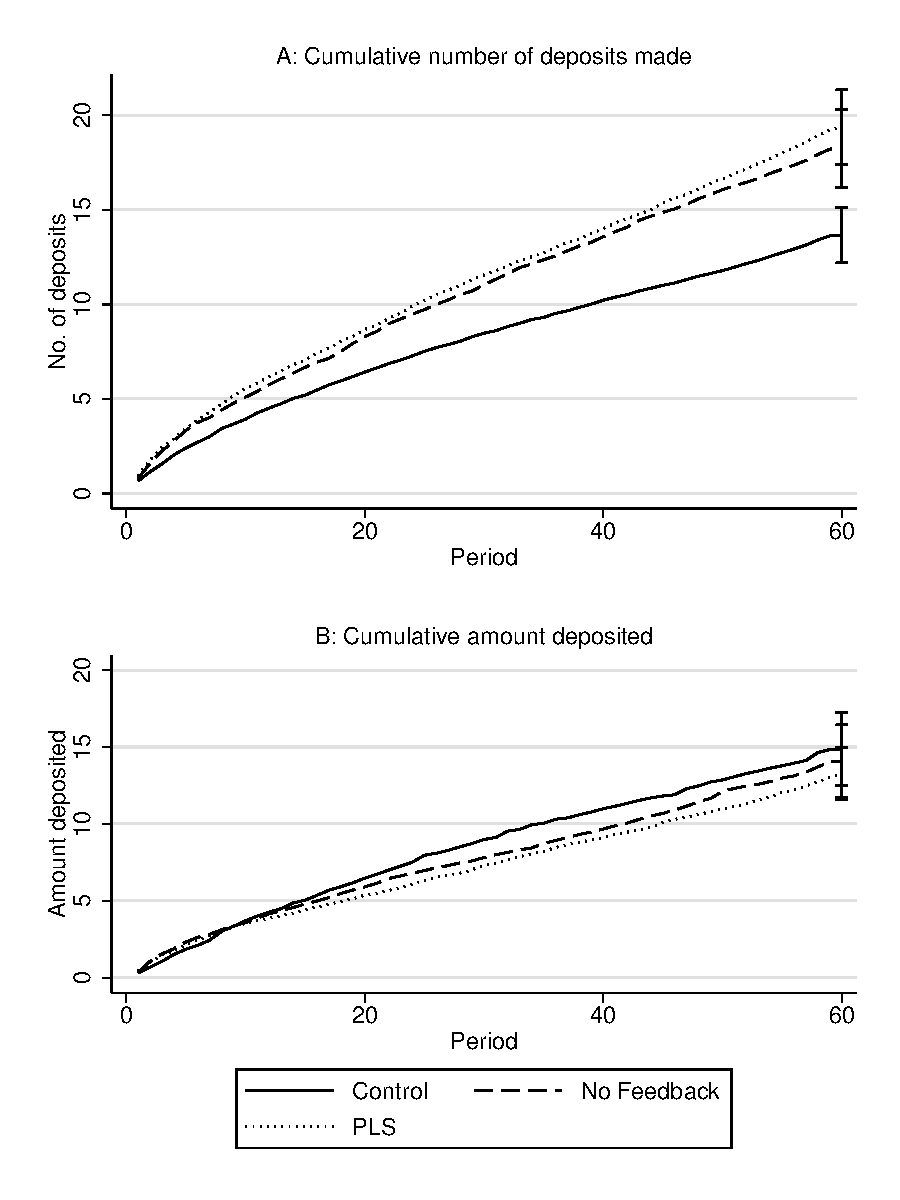
\includegraphics[height=0.85\textheight]{../../figures/line-cumdeposits.pdf}
			\label{fig:line-cumdeposits}
			\caption*{\footnotesize \emph{Notes:} Panel A plots the cumulative number of deposits made by the average participant over the 60-day savings period by treatment assignment. Panel B plots the cumulative amount deposited by the average participant. Error bars for totals by the end of the project are within one standard error of the group means.}
		\end{figure}

		\clearpage

		While effects on number of deposits are considerable, we find no effect of either PLS treatment on total amount deposited over the project period. Panel B of Figure \ref{fig:line-cumdeposits} plots the cumulative deposit amounts, averaged by treatment group, over the 60-day period. We cannot distinguish total deposit amounts between any of the three incentive schemes. Participants in the PLS group withdrew a larger amount relative to the control on average ($\hat \beta = 1.63, p < 0.05$) but we are unable to detect statistically significant differences in the final balance across treatment groups.

		Our results are consistent with a general finding among earlier field experiments on lottery-based incentives that behavioral responses occur on the extensive, but not intensive, margin. \textcite{brune_effect_2015} test a stochastic incentive in Malawi wherein tea harvesters entered a lottery conditional on attendance and could increase their probability of a prize according to their output. That study found significant improvements in workplace attendance, allowing workers to enter the lottery, but without changes in output. \textcite{loibl_testing_2016}, examined features of the Individual Development Account program in the U.S. and found no effect of PLS over certain returns of equal expected value. A recent experiment by \textcite{gertler_long-term_2017} randomized the provision of PLS across banks in Mexico and observed a 43\% increase in the number of account openings in the month the lotteries were in effect but without affecting balances.\footnote{\textcite{gertler_long-term_2017} observes effects on account openings but not on transactions compared to the control group. Our study opened accounts for all participants in the sample.}

		Other experimental results, which \emph{do} find effects on savings amount are to some degree at odds with our own. \textcite{atalay_savings_2014} conducted an online portfolio-choice experiment in the U.S. that resulted in subjects saving an additional 12 percentage points more with prize-linked and regular savings than with regular savings alone. \textcite{dizon_leveraging_2016} replicate this design in an experiment conducted in Haiti and identify a 22\% increase in savings.\footnote{\textcite{dizon_leveraging_2016} emphasize that savings responded to the presence of the stochastic component rather than expected returns.} In an experiment with undergraduates, \textcite{filiz-ozbay_lottery_2015} found that subjects are willing to accept a lower rate of return to delay a payment when the return is stochastic than when it is deterministic. The experimental design of these three studies differed from this one in two respects. First, subjects in those lab studies were supplied with an endowment with which to make portfolio allocations. With a median monthly income of USD 77, households in our study may be too liquidity constrained to sustain a larger balance with PLS. Baseline correlations suggest that monthly income is predictive of savings in the mobile product, though we do not observe heterogeneity of the treatment effect conditional on income. Second, our sample already had access to a number of competing savings products, both formal and informal, which could have dampened demand for PLS savings. Certainly, this discussion does not preclude other factors which could affect the external validity of the results presented here.

		% Dizon does not give feedback, Filiz-Ozbay does not, Brune no, Atalay no, Nyqvist no, Loibl no. So regret aversion can't actually explain prior results. Furthermore, it cannot be a mechanism behind those. The only thing we can say is that it could be used to encourage more saving.

		% Adrian's point about what we should expect people to do at the end of the savings period (put everything and leave), what happens during withdrawals, what does it mean for people to increase deposits but not savings, what the estimand is if preferences aren't stable.

		% In general, what should we expect as we get closer to a date of withdrawal? That savings should be high because discounting isn't as intense. This is not the case. Figure out what's going on.

	\subsection{The Role of Regret Aversion}

		That potential savers respond to PLS by making more frequent deposits without a corresponding increase in balance can be partially rationalized as the subdivision of lotteries to reduce risk \parencite{samuelson_risk_1963}. Under this hypothesis, risk averse individuals will subdivide bets over a greater number of gambles so that the risk of a low return is minimized. Since PLS offers returns equivalent in expectation to the matching incentive, we would expect risk averse individuals to save no more with PLS than with the standard account even without liquidity constraints. Yet another explanation for our findings is the ``entertainment'' utility hypothesis of gambling \parencite{conlisk_utility_1993}. That is, consumers will behave in ways that enable them to make gambles because they derive consumption utility from simply playing and irrespective of potential earnings. Under this hypothesis, an increase in the number of deposits in the treatment group is expected if merely making a deposit on a certain day qualifies participants to play the lottery for that day. Recall that participants had almost five more active days---and thus play the lottery five more times---than the control group. Unsurprisingly, participants are not making more deposits \textit{within} days since this does not affect lottery eligibility. For these reasons we expect the PLS to induce more deposits without a corresponding increase in amount saved.

		% consider moving the following section to the empirical strategy part

		Our study was designed to investigate the role of regret aversion as a specific mechanism explaining demand for PLS. Regret theory is a class of behavioral models that incorporate an individual's aversion to feelings of regret---an emotional response to foregone opportunities due to action or inaction. \textcite{bell_risk_1983} and \textcite{loomes_regret_1982} were one of the first to formalize this as a complication to expected utility theory. Where expected utility depends only on final outcomes, (dis)utility from regret (rejoicing) depends on the difference between the realized outcome and the best foregone outcome. Additionally, regret theory assumes that individuals can anticipate the psychological consequences of the decisions and therefore take them into account ex ante. These class of theories received attention due to their ability to rationalize behavioral deviations from expected utility theory (e.g. the Allais paradoxes).

		\textcite{zeelenberg_consequences_1996} and \textcite{zeelenberg_consequences_2004} demonstrate how the minimization of anticipated regret can rationalize risk-seeking behavior among risk-averse individuals in situations of \textit{asymmetric feedback}. This describes, for example, choices between a lottery and a certain outcome where choosing the lottery leads to its resolution whereas choosing certainty typically does not involve a resolution of the lottery. Since regret derives from a comparison of foregone outcomes, choosing the lottery and receiving feedback involves the possibility of regret while choosing certainty does not. A regret-minimizing individual would thus find certainty favorable above and beyond her risk preferences. Conversely, providing feedback on the lottery regardless of choice (a situation of \emph{symmetric feedback}), removes the role of regret aversion associated with certainty. \textcite{zeelenberg_consequences_1996} introduced the central test for regret aversion based on this observation. It involves comparing choices between situations of asymmetric versus symmetric feedback, \textit{ceteris paribus}, in order to isolate the role of regret aversion. 

		% this argument probably reqires formalization  
		% it's more like *without* regret aversion we would see greater effects.

		We adapt this test in our own experiment as a way of quantifying the contribution of regret aversion in the demand for PLS. Recall that in the PLS treatment, the lottery involves no possibility of losses and that lotteries are resolved regardless of saving. Therefore, regret manifests when individuals choose not to save but learn about foregone winnings from the lottery. Regret-minimization predicts that individuals on the margin make deposits (and enter the lottery) in avoidance of this regret. We compare behavior with an alternate PLS treatment (the No Feedback group) which provided a day's lottery results if and only if the individual made a deposit on that day. Participants in this condition correctly anticipate that choosing not to save involves no regret since they can remain unaware of their foregone lottery earnings. As a result, regret theory predicts greater deposits with feedback than without. Moreover, the difference in outcomes between the two treatments can be attributed to regret aversion alone. 

		Column 1 of Table \ref{tab:reg-fwermobile} shows that the effect of No Feedback on the number of deposits are positive but smaller in magnitude to the effect of PLS and are not significant at the 5\% level ($\hat \beta = 4.59, p < 0.10$). Column 3 reports on the difference between the PLS and No Feedback conditions, which we do not find statistically significant. The effect of No Feedback on number of days saved follows a similar pattern ($\hat \beta = 3.93, p < 0.10$) compared to PLS with feedback. Our estimates imply that approximately 20\% of the PLS treatment effect can be attributed to regret aversion.

	\subsection{Does Experienced Regret Affect Savings?}

		% motivate this better

		In the theory of regret outlined in the previous section, the anticipation of regret determines ex ante choice. That model makes no predictions regarding the role of recently experienced regret in individual choice. If participants feel the sting of foregone lottery winnings from yesterday, are they more likely to act on their regret aversion today?

		We can leverage the panel structure of our data and the randomness of the lottery results to estimate the effect of recently experienced regret on deposits. If participants are saving in response to experienced regret of foregoing the prize, we expect to see an independent effect of winning the lottery among non-savers on the decision to save in the PLS group. Let $Y_{i,t}$ denote having made a deposit by participant $i$ in period $t$. $\text{Win}_{i,t}$ is an indicator for having a winning lottery ticket from the pervious day announced in period $t$. We estimate the following equation conditional on assignment to the PLS group and not having saved one period prior.

		\begin{equation} \begin{split}
		Y_{i,t} = & \pi \text{Win}_{i,t} + \omega_{t} + u_{i,t}
		\end{split} \label{eq:regret} \end{equation}

		$\pi$ is the additional effect from winning but not being able to claim the prize. $\omega_{t}$ is a period-specific fixed effect. We test the null hypothesis of $\pi = 0$.

		\begin{table}[ht]\centering \def\sym#1{\ifmmode^{#1}\else\(^{#1}\)\fi} \caption{Regression of deposits on lottery results} \label{tab:reg-regretaversion} \maxsizebox*{\textwidth}{\textheight}{ \begin{threeparttable} \begin{tabular}{l*{2}{c}} \toprule
                &\multicolumn{1}{c}{Made a deposit}\\
\midrule
Winning ticket  &     0.02\sym{**} \\
                &   (0.01)         \\
\midrule
Adjusted \(R^{2}\)&    0.081         \\
Control mean    &     0.20         \\
Daily PLS effect&                  \\
Observations    &     4473         \\
\bottomrule \end{tabular} \begin{tablenotes}[flushleft] \footnotesize \item \emph{Notes:} This table reports on a regression of having saved at period \(t\) on winning the lottery at \(t\) conditional on being in the PLS group and not having saved at \(t-1\). The unit of observation is individual-by-period. The regression includes period fixed effects. Standard errors are in parentheses and clustered at the individual level. * denotes significance at 10 pct., ** at 5 pct., and *** at 1 pct. level. \end{tablenotes} \end{threeparttable} } \end{table}

% File produced by akiba-estimate.do with /Users/justin/Repos/akiba-lottery-pub/data/clean/akiba_long.dta on 11:52:17 25 Oct 2020 by user justin on Stata 13.1 with seed Xd950c82044e7d5a124b5a3e57a7d26c000042a30

		Table \ref{tab:reg-regretaversion} shows that the treatment effect is 2 percentage points ($p<0.05$) higher after learning about a winning ticket than learning about a losing one. With an average daily effect of 0.08 of PLS, this account for a fourth of the group treatment effect. Additional evidence comes from Figure \ref{fig:hist-deposits}, which plots the distribution of deposits over time and shows timing suggestive of regret aversion. Nearly all deposits made in the PLS group ocurred within an hour of announcing the lottery results from the previous day. We observe no similar pattern in the No Feedback and control groups. Together, the evidence suggests that recently experienced regret from foregone earnings improves the likelihood of entering the lottery in subsequent rounds.

		\begin{figure}[ht]
		\centering
		\caption{Timing of deposits}
		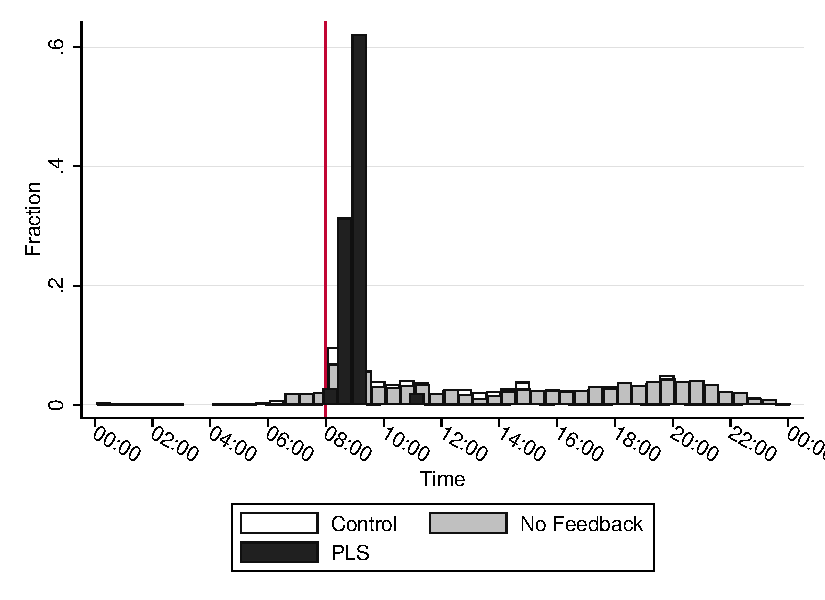
\includegraphics[width=\textwidth]{../../figures/hist-deposits.pdf}
		\label{fig:hist-deposits}
		\caption*{\footnotesize \emph{Notes:} This figure plots the empirical distribution of timing of all deposits over the project period. Each bin spans 30 minutes with a height equal to the fraction of all deposits within each treatment group. A vertical line marks 8:00, when participants received the first SMS that summarized how much the participant saved the previous day, how much the participant earned through a matching contribution or winnings, and their total balance. An hour later, participants received a second SMS encouraging them to save that day. Participants in PLS received a new lottery ticket with the second message.}
		\end{figure}

		\clearpage

	% \subsection{Effect on Deposits Persists Over Time}
	%
	% 	The preceding results provide evidence that PLS with feedback compels individuals to make more frequent deposits.
	%
	% 	We additionally find no statistically significant heterogeneity by interacting the treatment effect with period indicators.

		% we do not find evidence that this decreases (except after the first few days)

		% this has been documented in the lab with small stakes and repeated decisions. erev demonstrates that people who take median 15 (weber 2007 17) with replacement are less likely to overweight rare events. also erev speculates that this is through experience with the rare event and demonstrates it.
		% alternatively, overweighting of recent evidence. does winning affect decision to play in this study?
		% can subjective bias be decreasing over time? (zia paper)
		% brune paper on time dependence
		% which mechanisms are being activated? debiasing, overweighting of recent evidence

		% \begin{table}[ht]\centering \def\sym#1{\ifmmode^{#1}\else\(^{#1}\)\fi} \caption{Time-varying treatment effects on deposits} \label{tab:reg-timedummy} \maxsizebox*{\textwidth}{\textheight}{ \begin{threeparttable} \begin{tabular}{l*{2}{c}} \toprule
                &\multicolumn{1}{c}{Made a deposit}\\
\midrule
Lottery         &     0.10         \\
                &   (0.07)         \\
Regret          &     0.12\sym{*}  \\
                &   (0.07)         \\
Constant        &     0.60\sym{***}\\
                &   (0.05)         \\
\midrule
Adjusted \(R^{2}\)&    0.049         \\
Lottery joint \(p\)-value&     0.02         \\
Regret joint \(p\)-value&     0.01         \\
Observations    &    18660         \\
\bottomrule \end{tabular} \begin{tablenotes}[flushleft] \footnotesize \item \emph{Notes:} This table reports a regression of having saved at period \(t\) on treatment indicators interacted with period indicator variables. The unit of observation is individual-by-period. Standard errors are in parentheses and clustered at the individual level. * denotes significance at 10 pct., ** at 5 pct., and *** at 1 pct. level. \end{tablenotes} \end{threeparttable} } \end{table}

% File produced by akiba-estimate.do with /Users/justin/Repos/akiba-lottery-pub/data/clean/akiba_long.dta on 00:16:38 13 Jun 2019 by user justin on Stata 13.1 with seed X32b3301a224bcb612cd99bbd84ad23ad0004026c

		% \begin{figure}[ht]
		% \caption{Effects over time -- Number of deposits}
		% 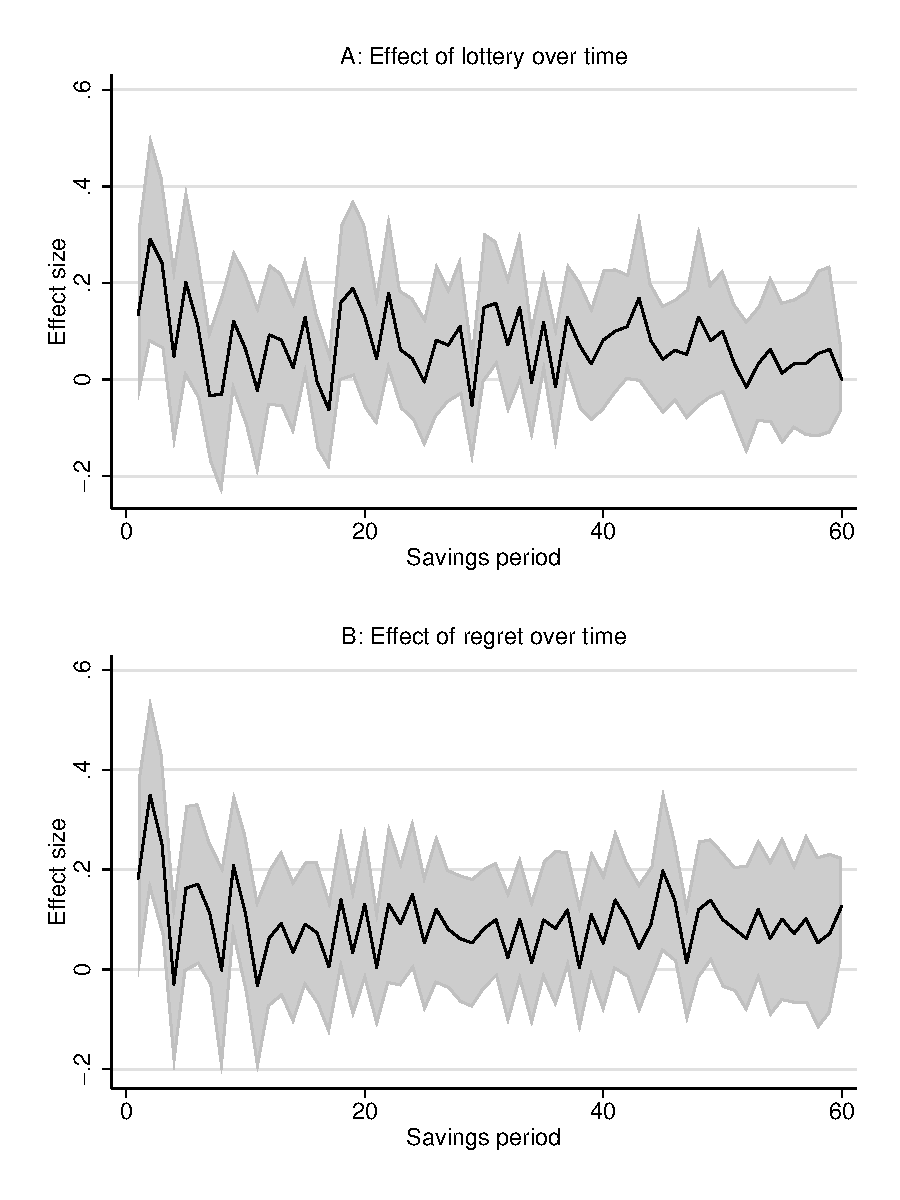
\includegraphics[width=\textwidth]{../../figures/line-timemobile_deposits.pdf}
		% \caption*{\footnotesize \emph{Notes:} Panel A plots the treatment effect of Lottery on number of deposits as a function of savings period. Panel B plots the treatment effect of PLS on number of deposits as a function of savings period. Shaded areas represent period-specific 95\% confidence regions.}
		% \end{figure}

	\subsection{The Effect of PLS on Savings by Other Means}

		% why would they be complements?

		A related objective of this study is to examine whether PLS act as complements or substitutes to existing savings products. Unsurprisingly, we do not find evidence that PLS crowds out saving by other means since there was no treatment effect on amount saved using PLS. Table \ref{tab:reg-fwersave} reports no statistically significant effect on total saving through M-Pesa or ROSCAs. We do find, however, that respondents in PLS are 14 percentage points ($p < 0.05$) more likely to save with a ROSCA compared to the control group and 16 percentage points ($p < 0.05$) more likely relative to the No Feedback condition. This result is robust to the inclusion of covariates but is significant at the 10\% level when correcting for multiple inference ($p < 0.10$). We find no effect of the No Feedback condition on informal saving. This finding is puzzling but one possible explanation is that participants may be borrowing from ROSCAs in order to fund their PLS deposits. Overall, we do not find that PLS cannibalizes savings from other sources in line with earlier experimental results \parencite{atalay_savings_2014,filiz-ozbay_lottery_2015,dizon_leveraging_2016}.

		\begin{table}[ht]\centering \def\sym#1{\ifmmode^{#1}\else\(^{#1}\)\fi} \caption{Treatment effects -- Savings outside the project} \label{tab:reg-fwersave} \maxsizebox*{\textwidth}{\textheight}{ \begin{threeparttable} \begin{tabular}{l*{5}{c}} \toprule
          &\multicolumn{3}{c}{Effect estimates}&\multicolumn{2}{c}{Sample}\\\cmidrule(lr){2-4}\cmidrule(lr){5-6}
          &\multicolumn{1}{c}{(1)}&\multicolumn{1}{c}{(2)}&\multicolumn{1}{c}{(3)}&\multicolumn{1}{c}{(4)}&\multicolumn{1}{c}{(5)}\\
          &\multicolumn{1}{c}{Lottery}&\multicolumn{1}{c}{Regret}&\multicolumn{1}{c}{\specialcell{Regret-\\Lottery}}&\multicolumn{1}{c}{\specialcell{Control Mean\\(SD)}}&\multicolumn{1}{c}{Obs.}\\
\midrule
Total savings last month&    18.45&   -17.87&   -36.32&    80.31&      284\\
          &  (25.16)&  (14.64)&  (24.06)& (112.74)&         \\
          &   [1.00]&   [1.00]&   [0.20]&         &         \\
M-Pesa savings last month&    -5.42&    -6.71&    -1.29&    20.42&      284\\
          &   (6.34)&   (5.49)&   (5.30)&  (44.67)&         \\
          &   [1.00]&   [1.00]&   [1.00]&         &         \\
ROSCA savings last month&     1.48&     7.37&     5.89&    22.24&      283\\
          &   (6.76)&   (6.79)&   (7.33)&  (42.18)&         \\
          &   [1.00]&   [1.00]&   [0.40]&         &         \\
Saves with a ROSCA&    -0.02&0.14\sym{**}&0.16\sym{**}&     0.54&      284\\
          &   (0.07)&   (0.07)&   (0.07)&   (0.50)&         \\
          &   [1.00]&   [0.40]&[0.00\sym{***}]&         &         \\
\bottomrule \end{tabular} \begin{tablenotes}[flushleft] \footnotesize \item \emph{Notes:} Columns 1--3 report OLS estimates of the treatment effect. Standard errors are in parentheses and FWER adjusted \(p\)-values are in brackets. Observations are at the individual level. * denotes significance at 10 pct., ** at 5 pct., and *** at 1 pct. level. Stars on the coefficient estimates reflect unadjusted \(p\)-values. \end{tablenotes} \end{threeparttable} } \end{table}

% File produced by reg-fwer.do with /Users/justin/Repos/akiba-lottery-pub/data/clean/akiba_wide.dta on 00:15:52 13 Jun 2019 by user justin on Stata 13.1 with seed X27e0a1708256a41cdeaf4038df2ac2a9000400f4

	\subsection{PLS Increases Self-Reported Gambling}

		% why would they be complements?

		At the end of the trial, we asked participants whether they gambled more than they usually do apart from participating in the savings program. As reported in Table \ref{tab:reg-fwergamble}, we find that participants in the PLS group self-report higher gambling behavior the savings program. On average, treated participants are 15 percentage points ($p < 0.05$) more likely to report gambling than the control group. This finding is robust to covariate ajdustment and is significant at the 10\% level after FWER adjustment. We find no average effects for participants in the No Feedback group. Our measure for gambling activity is susceptible to experimenter demand though it is unclear in what direction this might bias our estimate. With this caveat in mind, the effect provides some evidence of a complementary relationship between PLS and broader gambling behavior.

		\textcite{atalay_savings_2014} and \textcite{dizon_leveraging_2016} both observe large reductions in gambing expenditure in order to finance savings with PLS. It is possible that while PLS is a substitute for gambling with a cash windfall (as in their study), it interacts differently when indviduals already have a history of gambling. \textcite{cookson_when_2016} offered individuals in Nebraska access to an PLS and observed cash withdrawals at casinos as a measure of gambling behavior. They find reductions in transactions between 7-15\% and credit the effect to substition of casino gambling with PLS.

		\begin{table}[h]\centering \def\sym#1{\ifmmode^{#1}\else\(^{#1}\)\fi} \caption{Treatment effects controlling the FWER -- Gambling} \label{tab:reg-fwergamble} \maxsizebox*{\textwidth}{\textheight}{ \begin{threeparttable} \begin{tabular}{l*{5}{c}} \toprule
          &\multicolumn{3}{c}{Effect estimates}&\multicolumn{2}{c}{Sample}\\\cmidrule(lr){2-4}\cmidrule(lr){5-6}
          &\multicolumn{1}{c}{(1)}&\multicolumn{1}{c}{(2)}&\multicolumn{1}{c}{(3)}&\multicolumn{1}{c}{(4)}&\multicolumn{1}{c}{(5)}\\
          &\multicolumn{1}{c}{Lottery}&\multicolumn{1}{c}{Regret}&\multicolumn{1}{c}{\specialcell{Difference\\\(p\)-value}}&\multicolumn{1}{c}{\specialcell{Control Mean\\(SD)}}&\multicolumn{1}{c}{Obs.}\\
\midrule
Gamble more&     0.06&0.15$^{***}$&     0.16&     0.12&      284\\
          &   (0.05)&   (0.06)&         &   (0.32)&         \\
          &   [0.61]&[0.05]$^{*}$&         &         &         \\
Gamble less&    -0.02&     0.04&     0.24&     0.16&      284\\
          &   (0.05)&   (0.06)&         &   (0.37)&         \\
          &   [0.88]&   [0.80]&         &         &         \\
More tempted to gamble&     0.09&     0.05&     0.56&     0.47&      284\\
          &   (0.07)&   (0.07)&         &   (0.50)&         \\
          &   [0.61]&   [0.80]&         &         &         \\
Less tempted to gamble&    -0.01&     0.03&     0.27&     0.06&      284\\
          &   (0.03)&   (0.04)&         &   (0.25)&         \\
          &   [0.88]&   [0.80]&         &         &         \\
\bottomrule \end{tabular} \begin{tablenotes}[flushleft] \footnotesize \item \emph{Notes:} Columns 1--2 report OLS estimates of the treatment effect. Column 3 reports the \(p\)-values for tests of the equality of the two treatment effects. Standard errors are in parentheses and FWER adjusted \(p\)-values are in brackets. Observations are at the individual level. * denotes significance at 10 pct., ** at 5 pct., and *** at 1 pct. level. Stars on the coefficient estimates reflect unadjusted \(p\)-values. \end{tablenotes} \end{threeparttable} } \end{table}

% File produced by reg-fwer.do with /n/homeserver2/user2a/justinra/repos/akiba-lottery-pub/data/clean/akiba_wide.dta on 02:33:07 16 Feb 2018 by user justinra on Stata 13.1 with seed X71d1d353b37e281e006fa26738e26f4500044a1c

\section{Conclusion} \label{sec:conclusion}

	There is an abundance of evidence on the promise of product design in encouraging savings among the poor. We conducted a randomized experiment testing a prize-linked savings product with informal residents in Nairobi, Kenya. Utilizing a mobile savings platform, we randomly assign respondents to a savings account with a certain, matching incentive, a lottery incentive, and a lottery incentive with feedback on ex post potential lottery winnings. We set the fixed match of 5\% equivalent in expectation to the lottery prize so that comparing the two groups identifies the effect of stochastic incentives compared to deterministic incentives. After observing account transactions over a 60-day savings period, we find that participants in the PLS group made between 5-6 more deposit transactions than the matched payments group without a corresponding increase in amount saved. We further find no effects on amounts saved through other channels except that participants assigned to the PLS treatment with feedback were 14 percentage points more likely to have saved with a ROSCA.

	Comparing the two PLS treatments provides a test of regret aversion as an underlying mechanism behind the increased usage that we observe. Under this hypothesis, marginal savers will be induced to make deposits in order to minimize the anticipated regret from missing out on the prize. Our findings are consistent with regret minimization: individuals make 20\% more deposits when they expect to be given feedback about lottery results regardless of their decision to save. Participants in the feedback condition are also 8\% more likely to make a deposit as a result of having recently won a lottery without a prize. Our intepretation for this result is that recently experienced regret may intensify aversion to anticipated regret and further motivate deposits.

If PLS contribute to problem gambling, the program is potentially welfare-decreasing for households susceptible to problem gambling. 

PLS may thus improve utilization among existing account holders and be able to attract new savers to open formal savings accounts. Frequent deposits may also have long-term benefits by encouraging the formation of a savings habit \parencite{alessie_saving_2009}. From a policy perspective, PLS may not be revenue neutral compared to matching if financial institutions incur greater transaction costs as a result of more frequent deposits.

If PLS increase deposits but are ineffective at increasing a key outcome like savings, are they still useful from a policy perspective? If playing the lottery is appealing to potential savers, PLS may be able to attract new savers to open  accounts. PLS can also improve utilization among existing account holders. Frequent deposits may have long-term benefits by encouraging the formation of a savings habit \parencite{alessie_saving_2009}. Compared to a fixed match, lottery incentives may not be revenue neutral if financial institutions incur greater transaction costs as a result of more frequent deposits. If PLS contribute to problem gambling, the program is potentially welfare-decreasing for poor households already susceptible to costly gambling behavior. Overall, we document important differences between PLS and fixed-incentive schemes when it comes to encouraging savings and show that product design is crucial in determining welfare implications.

		% reference long term studies (gertler, schaner) as well as the default effect one (somville)
		% discussion about revenue neutrality is part of a larger cost-effectiveness analysis 

		% \parencite{gertler_long-term_2017}: We observe the opposite: although initially lower, the savings balances of  compliers  who open accounts in response to the incentive catch up to the savings balances of those who open accounts in control branches. The levels of active use of the account are similar across lottery month account openers in treatment and control branches.
		% Focus on a potentially important outcome (no. of deposits/streak) determining long-term savings behavior previously neglected in the literature (Less than 20\% of banked adults in Sub-Saharan Africa make more than 2 deposits in a month \parencite{demirguc-kunt_global_2015})
		% This may be an effective tool to encourage savings on the _extensive_ margin
		% brune's point about temporary vs persistent preferences implications for policy
		% Can we target better? Working poor, emerging middle class, the present study's het effects
		% Effects on downstream outcomes (consumption, etc.)
		% Tighter accounting to track savings and expenditure
		% We didn't really ask about savings goals
		% Should have incorporated higher order risk preferences (CPT)
		% Would have been good to analyze how intensity of regret aversion affects the decision to save (can't because ticket generation suffers from selection)
        % Might want to test variation in skewness holding spread constant
		% Our results target a specific behavior: people who have savings account but don't use them
		% demand is strong (tufano/cole) but actually people don't save more (it doesnt meet policy goals exactly) (it is not straightforward to justify PLS as a policy tool on the basis of demand)
		% should have also run a pure regret treatment arm to separate out effects

\newpage

\printbibliography

% Our contributions:
%
% 	causal evidence of PLS on savings and gambling
% 	Developing country setting
% 	Mobile savings allow tight tracking of savings behavior
% 	Multi-period panel setting gives us dynamic information (Samuelson)
% 	Test the influence of regret aversion
% 	Focus on a potentially important outcome (no. of deposits/streak) determining long-term savings behavior previously neglected in the literature (Less than 20\% of banked adults in Sub-Saharan Africa make more than 2 deposits in a month \parencite{demirguc-kunt_global_2015})
% 	The effect of PLS remains unclear, so we help understand through what channels PLS affects what
%
% Notes:
%
% 	no matter how much we dig into panel, a qje paper is not coming out because of our results, more refined story rather than extra analysis
% 	its promising as a great example of a null result, what are some theories about why this didnt work? i mean its a huge match so we set ourselves up for failure, theres already a ceiling effect
% 	MA: survey experiment prior duke MBA students get theory from this, lotteries work well when the interest rate is low but not as it increases
% 	think about intertemporal consumer behavior; what does it predict?; what do our results say about the prevailing model?

\end{document}
